\chapter{Categorical Perception}

\section{Introduction}
\subsection{What is categorical perception?}

\CP occurs when categories held by the observer, either learned or inherent, influence the observer’s perception. This means that the perception of changes in the stimuli does not depend solely on the physical changes in the stimuli. Small changes in stimuli that lie near or across category boundaries are very noticeable while larger changes in other regions may not be noticeable at all. This means that our perceptual systems transform relatively linear sensory signals into relatively nonlinear internal representations.

\begin{figure}[h] 
  \centering
  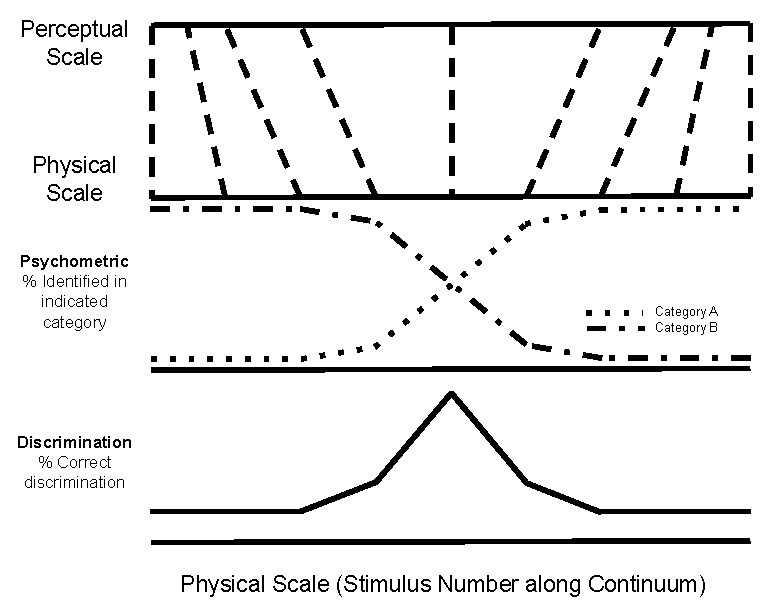
\includegraphics[width=0.75\textwidth]{figures/CP_def.pdf}
  \caption[A schematic of idealized categorical perception]
{A schematic of idealized categorical perception. \emph{Top}: The lower scale depicts a series of stimuli that are spaced a fixed distance apart according to some physical measure. In a perceptual representation of these stimuli the distances between adjacent stimuli may be modified in a way that groups the stimuli into categories as shown in the upper scale. \emph{Middle:} Idealized psychometric function or identification functions to illustrated the categorical perception of the nine stimuli distributed at equal intervals along the physical continuum. This is the percent identified in the indicated category plotted against the the stimulus number along the continuum, i.e. the physical scale. \emph{Bottom:} Discrimination function representing the increased sensitivity to changes in the stimuli near the categorical boundary.\index{cp}}
  \label{fig:cpdef}
\end{figure}

\subsection{Why European Starlings?}

\subsection{What is required for \CP research?}

The fundamental difficulty with \CP research is that it generally occurs in the perception of a high dimensional space where naturally occurring ecologically relevant stimuli exist only on non-uniformly distributed sub-manifold of that space. In terms of auditory \CP in human speech, the high dimensional space is the space of all possible sounds that could possibly be heard, most of which would sound like random noise. The naturally occurring ecologically relevant stimuli is all the possible spoken sounds or phonemes that are useful for human speech production and comprehension, which exist in a much smaller lower-dimensional subset of all possible sounds. Even within this subset of sounds, not all possible phonemes are heard with equal probability and this distributional information may begin to shape our perceptual systems even before birth.

Because of this, the majority of auditory \CP has focused on human speech sounds, predominantly English, leveraging our intuitions and years of linguistic modelling to identify the relevant dimensions where \CP occur. \CP work concerning animal vocalizations must first identify stimuli that are categorically perceived, a process that was very labor intensive\cite{swamp sparrow series of papers} before the development of more modern techniques\cite{Tim's paper on distribution}. The variation within the songs of European starlings also make this easier because it is much easier to find song elements that are of distinct types.

Furthermore, the identification of category boundaries is more difficult in non-human research than with human subjects. Since we can't provide instructions, we are forced to use multiple shaping or pre-training stages of operant behavioral conditioning. Also, if we permit a fully adaptive double staircase procedure, our subjects learn to exploit this and force the boundary all the way to one side or another. To solve this we use a new staircase technique.

Last, but certainly not least, \CP requires the generation of a synthetic continuum between the categories or category exemplars. In human speech, the existence of speech synthesizers has made this task easy, at least in English. In Chinese for example, the technical difficulty in creating a Chinese-based synthetic continuum suitable for a \CP study has been proposed as a reason for the large number of papers focused on \CP in lexical tones in the Chinese language\cite{zhang2013categorical}. \CP research on animal vocalization has been limited to exploiting natural variation in recorded calls\cite{swamp sparrow cp} which invariably limits the sampling and control over the stimuli. It has also been shown that the quality of the speech synthesizer is correlated with how much \CP is observed\cite{something}.

Thus the approach we present streamlines the following steps for \CP research:
Identification of relevant dimensions where \CP occurs
Identification of categorical boundaries
Generation of a synthetic continuum between the categories/ category exemplars.

\subsection{History of Categorical Perception}

There is a long history of categorical perception research.

The invention of the formant speech synthesizer known as the Pattern Playback at Haskins Laboratories\cite{patternplayback} made the discovery of \CP possible.
The Pattern Playback was a machine that converted pictures of the acoustic patterns of speech in the form of a spectrograms into sound using light.

\CP was initally described as the absolute definition of completely quantal perception where subjects would be unable to discriminate differences to stimuli within a category, only noticing differences in stimuli that lies across category boundaries\cite{liberman1957discrimination, Studdert1970motor}. Although only ever described as an idealized case, this definition is far too restrictive and has been disproven many times, however, it has caused much criticism of the work done in the \CP field with critics calling for ``The end of categorical perception as we know it''\cite{schouten2003end} etc.

Later work has instead demonstrated that with-category differences are discriminable\cite{pisoni1974reaction,carney1977noncategorical,massaro1983categorical} and meaningful\cite{miller1997internal,mcmurray2002gradient,mcmurray2008gradient}. Thus it seems there is just an increase in sensitivity to differences in stimuli that lie across category boundaries.

\CP first explored in 1957 concerning the discrimination of speech sounds within and across phenome boundaries\cite{liberman1957discrimination}.  In addition to dubbing the term ``Categorical Perception,'' Liberman suggested that \CP was unique to human speech, and furthermore, was what made human speech special. He also originally proposed the motor theory of speech perception\cite{liberman1967perception}.

Formerly thought to be peculiar to speech and color perception, \CP turns out to be far more general and may be a result of the way our neural circuits are wired to identify hierarchical patterns.

\CP also provides an intermediate explanation of equivalence classes which in turn form the basis of high-level symbolic thought.
Auditory \CP also forms the basis for human language

Previously thought auditory \CP to be strictly human trait possibly depending on special processing or that there might be some sort of motor theory basis that could inform perception based on a motor production model.
Now thought to be a ubiquitous feature of all perceptual systems.

It has been shown in chinchilla\cite{kuhl1975speech} and later in macaques\cite{kuhl1983enhanced}, that animal models also have enhanced discriminability at human phonetic boundaries without a phylogenetic history of phenomic knowledge, either acoustic or articulatory.
These studies consists of playing human speech sounds to animals and behaviorally measuring if they place the same boundaries we do.
This has been used to argue that human languages may have adapted to use phenome category boundaries located in regions with intrinsically higher discriminability\cite{stevens1981constraints,goldstone2010categorical}

There also exists a host of research on \CP in non-human vocal communication sounds. These studies either use
natural variation in the vocalizations
artificially generated hand drawn spectrogram morphs.
These studies are only possible after considerable background work establishes the relevant categories, similar to the techniques originally used in humans to identify \CP.

Categorical boundary location preference has also been explored, mostly in the context of human speech. Early explanations included the motor theory of speech perception which suggested that the explanation for \CP lay in the anatomy of speech production, specifically, physical differences during articulation\cite{liberman1967perception}. There have also been arguments made that a biological predisoposition influenced the development of human languages pushing phenome boundaries to locations of increased sensitivity\cite{stevens1981constraints, goldstone2010categorical, halle1979some}

\subsection{Learned Categorical Perception}

However, we also know that the boundary location is experience dependent. Native language exposure can shift boundary locations. Also, a sound difference that crosses a boundary of a language will be more discriminable to speakers of that language than to speakers of a language that doesn’t have a boundary in that location.

Lots more here about learning on \CP, also context dependency

\subsection{Our Contribution}
We use machine learning techniques to approximate unsupervised statistical learning of the distribution of the set of natural motifs while compressing it into a lower dimensional representation. This allows us to generate a continuum of synthetic motifs that lie between exemplars.

These types of machine learning methods allow for the creation of synthetic continua between exemplars when trained upon a corpus of that stimuli type. This allows for the exploration of natural ecologically relevant animal communication signals as we have done here. It also would allow the exploration of categorical perception in non-english languages. For example, technical difficulty in creating the Chinese-based synthetic continuum suitable for a \CP study has been proposed as a reason for the large number of papers focused on \CP in lexical tones in the Chinese language\cite{zhang2013categorical}.

Furthermore, stimulus naturalness has been shown to be a factor determining the degree of categorical perception, so as these machine learning techniques improve, we may be able to better explore the \CP phenomena.

This method allows for the creation or discovery of boundaries of \CP in an unsupervised way in animal vocalizations and are thus more ecologically relevant and will activate auditory regions that are specifically tuned to conspecific vocalizations.
